%%%%%%%%%%%%%%%%%%%%%%%%%%%%%%%%%%%%%%%%%%%%%%%%%%%%%%%%%%%%%%%%%%%%%%%%%%%%%%%
%%	Fichier	   : models.tex
%%	Auteur     : helfer@tfel001.cad.cea.fr
%%	Date       : 01 Feb 2008
%%%%%%%%%%%%%%%%%%%%%%%%%%%%%%%%%%%%%%%%%%%%%%%%%%%%%%%%%%%%%%%%%%%%%%%%%%%%%%%

%%\documentclass[rectoverso,index,leqno,anti,projet]{note_technique_2005}
\documentclass[a4paper,12pt]{article}
\usepackage{fullpage}

\usepackage[english,francais]{babel} 

\usepackage[utf8]{inputenc}
\usepackage[T1]{fontenc}

\usepackage{graphicx}
\usepackage{amsmath}
\usepackage{color}
\usepackage{highlight}

\usepackage{pstricks}
\usepackage{pst-node}
\usepackage{pst-blur}

\usepackage{longtable}
\usepackage{colortbl}
\usepackage{multicol}
\usepackage{pifont}
%\usepackage{couleurs}

%%\usepackage{mecanique}
%%\usepackage{presentation}
%%\usepackage{divers}
%%\usepackage{chimie}

\newcommand{\celaeno}{{\tt celaeno}}
\newcommand{\tfel}{Pléiades}
\newcommand{\pcheck}{{\tt tfel-check}}
\newcommand{\castem}{{\tt CAST3M}}
\newcommand{\nom}[1]{{\tt #1}}

\newcommand{\code}[1]{
  \psframebox[linecolor=orange,shadow=true,blur=true]{
    \begin{minipage}[htbp]{1.0\linewidth}
      \tt\small #1
    \end{minipage}
  }
}


%\resumecea{%%%%%%%%%%%%%%%%%%%%%%%%%%%%%%%%%%%%%%%%%%%%%%%%%%%%%%%%%%%%%%%%%%%%%%%%%%%%%%%
%%	Fichier	   : resume.tex
%%	Auteur     : helfer@tfel001.cad.cea.fr
%%	Date       : 01 Feb 2008
%%%%%%%%%%%%%%%%%%%%%%%%%%%%%%%%%%%%%%%%%%%%%%%%%%%%%%%%%%%%%%%%%%%%%%%%%%%%%%%

Les applications \tfel{} évoluent. Cette évolution est liée d'une part
au développement des applications elles-mêmes mais également au développement
de l'architecture \tfel{} et au renouvellement des différents pré-recquis
qu'elle utilise (compilateurs,support du format MED,\castem{},
{\tt py\castem{}}, etc.).

Comme tout développement informatique, ces évolutions peuvent conduire à des
modifications des résultats, même si les modèles physiques restent
{\em inchangés}. Ces modifications peuvent avoir plusieurs origines, nous pensons
notamment aux modifications des algorithmes numériques utilisés.

Cette note présente un outil, nommé {\tt tfel-check}, permettant
de contrôler de manière {\em automatisée} sur un ensemble de calculs de référence
que les évolutions des applications sont {\em stables}, c'est à dire
que les résultats ne sont que peu \og~perturbés~\fg, au sens d'une erreur
définie par le développeur. Cet outil s'intègre et renforce
la stratégie \og~qualité~\fg mise en place dans la plate-forme \tfel{}.

Cet outil a initialement été développé pour les besoins de l'application
\celaeno{}.

%%% Local Variables: 
%%% mode: latex
%%% TeX-master: t
%%% End: 
}

\title{\pcheck \\
\bigskip{}
Notice d'utilisation}
\author{Thomas \textsc{Helfer}, Stépane \textsc{Bernaud}, Rémy \textsc{Petkantchin}}

%         Commissariat à l'Énergie Atomique
%\parskip \baselineskip

\begin{document}
\maketitle
\abstract{%%%%%%%%%%%%%%%%%%%%%%%%%%%%%%%%%%%%%%%%%%%%%%%%%%%%%%%%%%%%%%%%%%%%%%%%%%%%%%%
%%	Fichier	   : resume.tex
%%	Auteur     : helfer@tfel001.cad.cea.fr
%%	Date       : 01 Feb 2008
%%%%%%%%%%%%%%%%%%%%%%%%%%%%%%%%%%%%%%%%%%%%%%%%%%%%%%%%%%%%%%%%%%%%%%%%%%%%%%%

Les applications \tfel{} évoluent. Cette évolution est liée d'une part
au développement des applications elles-mêmes mais également au développement
de l'architecture \tfel{} et au renouvellement des différents pré-recquis
qu'elle utilise (compilateurs,support du format MED,\castem{},
{\tt py\castem{}}, etc.).

Comme tout développement informatique, ces évolutions peuvent conduire à des
modifications des résultats, même si les modèles physiques restent
{\em inchangés}. Ces modifications peuvent avoir plusieurs origines, nous pensons
notamment aux modifications des algorithmes numériques utilisés.

Cette note présente un outil, nommé {\tt tfel-check}, permettant
de contrôler de manière {\em automatisée} sur un ensemble de calculs de référence
que les évolutions des applications sont {\em stables}, c'est à dire
que les résultats ne sont que peu \og~perturbés~\fg, au sens d'une erreur
définie par le développeur. Cet outil s'intègre et renforce
la stratégie \og~qualité~\fg mise en place dans la plate-forme \tfel{}.

Cet outil a initialement été développé pour les besoins de l'application
\celaeno{}.

%%% Local Variables: 
%%% mode: latex
%%% TeX-master: t
%%% End: 
}

\parskip=5pt
\section{Introduction}

Les applications \tfel{} évoluent. Cette évolution est liée d'une
part au développement des applications elles-mêmes mais également au
développement de l'architecture \tfel{} et au renouvellement des
différents pré-recquis qu'elle utilise (compilateurs,support du format
MED,\castem{}, {\tt py\castem{}}, etc.) ou au changement
d'architecture matérielle.

Comme tout développement informatique, ces évolutions peuvent conduire
à des modifications des résultats, même si les modèles physiques
restent {\em inchangés}. Ces modifications peuvent avoir plusieurs
origines, nous pensons notamment aux modifications des algorithmes
numériques utilisés. Ceci est d'autant plus vrai pour les applications
les moins matures, dont l'évolution est souvent très rapide. C'est le
cas par exemple de l'application \celaeno{}.

Afin de limiter de détecter des modifications trop importantes des
résultats, souvent signe d'une régression ou d'une erreur de
programmation, les applications \tfel{} ont mis en place des
calculs de référence. Les résultats de ces calculs, fixés au moment de la
stabilisation d'une version ou de leur qualification ou encore de leur
validation suivant les cas, servent de référence. La procédure
consiste alors à vérifier de manière plus ou moins périodique, que les
résultats obtenus par les applications sur ces calculs de référence
sont restés pratiquement inchangés par rapport aux résultats de
référence.

Cette manière de procéder souffre aujourd'hui de deux écueils~:
\begin{itemize}
\item les calculs de référence et les comparaisons doivent être
effectués à la main, ce qui est fastidieux~;
\item les comparaisons se basent essentiellement sur des vérifications
visuelles, par comparaison des fichiers résultats ou par tracer. Dans
le dernier cas, la précision est de l'ordre de taille du trait utilisé
pour le tracé.
\end{itemize}

\begin{figure}[htbp]
  \centering
  \begin{tabular}[htbp]{c}
    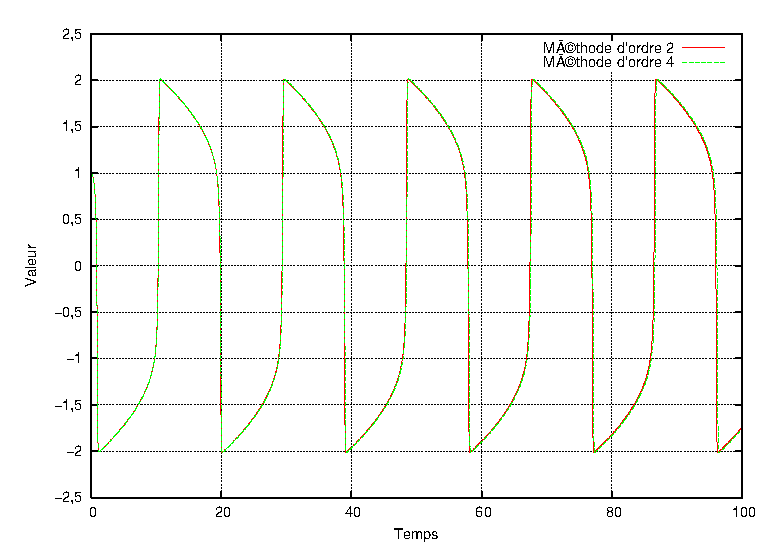
\includegraphics{Images/rk-results.eps} \\
    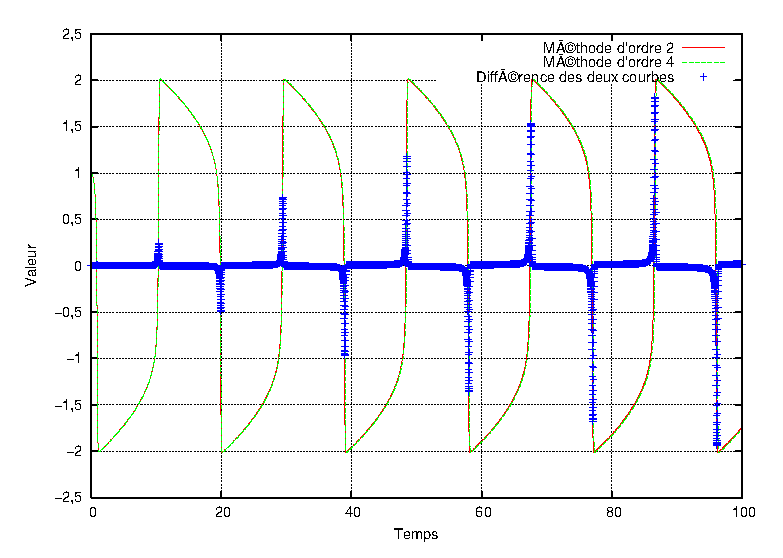
\includegraphics{Images/rk-results-errors.eps}
  \end{tabular}
  \caption{Imprécision liée à une vérification visuelle d'un résultat.}
  \label{fig:imprecision}
\end{figure}

Cette comparaison visuelle peut être trompeuse. Nous en avons fait
l'expérience en comparant les résolutions d'une même équation
différentielle avec une méthode de {\nom Runge-Kutta} d'ordre $2$
et avec une une méthode de {\nom Runge-Kutta} d'ordre $4$ (le pas de
temps est ici fixé, il ne s'agit pas de méthode à pas de temps
adaptatif). Cette comparaison est montrée en
figure~\ref{fig:imprecision}.

Le premier graphique montre des résultats extrêmement
semblables et il est difficile de distinguer les deux courbes. Le
second graphique trace, en plus de ces deux résultats, leurs
différences, c'est à dire l'erreur commise~: celle-ci atteint
pratiquement l'amplitude des oscillations au bout d'une dizaine de
périodes !

\subsection{Objet de cette note}

Nous avons développé, dans l'architecture 1.4, un outil, nommé {\tt
tfel-check}, permettant de vérifier de manière {\tt automatisée},
que l'ensemble des calculs de référence conduisent à des résultats
proches des résultats de référence. 

Cet outil reprend et généralise un ensemble d'outils développés par
ailleurs, pour la validation d'Alcyone par exemple.

La définition de l'erreur admissible, et le choix d'une méthode de
comparaison, relative ou absolue, doit être laissée à l'appréciation
des développeurs. Ainsi, il peut être raisonnable d'avoir une
précision absolue de quelques Pascals sur des valeurs de contrainte
et une précision relative de $10^{-8}$ sur les valeurs
du taux de combustion.

Cette note commence par détailler le principe de fonctionnement de
l'outil. La réalisation d'un cas de validation est détaillée en seconde
partie.

\newpage
\section{Principe de fonctionnement}

L'outil \pcheck{}, disponible dans l'architecture 1.4, se
lance sans argument.  Il parcourt l'ensemble des sous répertoires du
répertoire courant à la recherche de fichiers ayant l'extension
\og~{\tt .check}~\fg. La syntaxe de ce fichier est décrite en
section~\ref{sec:descr-du-fich}.

\pcheck{} se rend dans chaque répertoire contenant un fichier de
vérification, l'analyse. Si ce fichier contient une directive
de génération de maillage, celle-ci est effectuée. Si ce
fichier contient une directive d'exécution d'un calcul,
celle-ci est effectuée.

Cette éventuelle phase d'obtention de résultats étant
effectuée, \pcheck{} effectue l'ensemble des comparaisons demandées
dans le fichier de vérification. 

\pcheck{} effectue des comparaisons entre deux fichiers texte,
généralement le fichier contenant les résultats de référence et le
fichier contenant les résultats donnés par la version actuelle de 
l'application. Les comparaisons se font sur un ensemble de
{\em colonnes} de résultats. Les comparaisons se font valeurs par
valeurs de manière relative ou absolue. Le fichiers de résultats
doivent donc avoir un format particulier qui semble être celui
utilisé par l'ensemble des applications \tfel{}.

\subsection{Format des fichiers résultats}

Les fichiers résultats servant de base aux comparaisons doivent être
des fichiers texte et les résultats doivent apparaître sous forme de
colonnes. Les commentaires C/C++ sont ignorés. Les lignes commençant
par le caractère {\tt \#} sont ignorées.

Enfin, la première ligne, si elle est constituée de caractères
alphinumériques, pourra être utilisée comme entête des colonnes.

\subsection{Résultats de \pcheck{}}

Pour chaque fichier de validation, \pcheck{} affiche sur la sortie
standard une ligne indiquant le succès et l'échec de l'ensemble des
tests. Les figures~\ref{fig:pcheck-output-success}
et~\ref{fig:pcheck-output-failed} donnent un exemple d'affichage
pour chacun de ces cas.

\begin{figure}[htbp]
  \centering
  \code{
    ./tests/test-isotrope/celaeno.checkEx\mbox{ }\mbox{ }\mbox{ }\mbox{ }\mbox{ }\mbox{ }\mbox{ }\mbox{ }\mbox{ }\mbox{ }\mbox{ }\mbox{ }\mbox{ }\mbox{ }\mbox{ }\mbox{ }\mbox{ }\mbox{ }\mbox{ }\mbox{ }\mbox{ }\mbox{ }\mbox{ }\mbox{ }\mbox{ }\mbox{ }\mbox{ }\mbox{ }\mbox{ }\mbox{ }:\mbox{ }\textcolor{green}{[SUCCESS]}
  }
  \caption{Message de sortie en cas de succès d'un test.}
  \label{fig:pcheck-output-success}
\end{figure}

\begin{figure}[htbp]
  \centering
  \code{
    ./tests/test-isotrope/celaeno.checkEx\mbox{ }\mbox{ }\mbox{ }\mbox{ }\mbox{ }\mbox{ }\mbox{ }\mbox{ }\mbox{ }\mbox{ }\mbox{ }\mbox{ }\mbox{ }\mbox{ }\mbox{ }\mbox{ }\mbox{ }\mbox{ }\mbox{ }\mbox{ }\mbox{ }\mbox{ }\mbox{ }\mbox{ }\mbox{ }\mbox{ }\mbox{ }\mbox{ }\mbox{ }\mbox{ }:\mbox{ }\textcolor{red}{[FAILED]}
  }
  \caption{Message de sortie en cas d'échec d'un test.}
  \label{fig:pcheck-output-failed}
\end{figure}

\pcheck{} affiche un résumé des actions entreprises dans le fichier
\pcheck{}{\texttt{.log}}. Dans chaque répertoire contenant un fichier
de validation, \pcheck{} crée les fichiers suivants~:
\begin{itemize}
\item {\tt \$\{file\}-Mesh-<n>.out} contenant la sortie de la
  n\up{ième} génération de maillage~;
\item {\tt \$\{file\}-Exec-<n>.out} contenant la sortie du n\up{ième} calcul~;
\item {\tt \$\{file\}.checklog} contenant le résultat de tous les tests exécutés par \pcheck{}~;
\item {\tt TEST-\$\{file\}.xml} contenant le résultat de tous les tests exécutés par \pcheck{}~ au format JUNIT (pour intégration dans un outil d'intégration continue par exemple)~;

\end{itemize}

où {\tt \$\{file\}.check} est le nom du fichier de validation.

\newpage
\section{Description du fichier d'entrée}
\label{sec:descr-du-fich}

\newpage
\section{Description du fichier d'entrée (v1)}
\label{sec:descr-du-fich-v1}

\begin{figure}[htbp]
  \centering
  \code{
    \noindent
\ttfamily
\hlslc{// Meshing}\hspace*{\fill}\\
\hlstd{MeshCommand }\hlstr{'celaenoMesh {-}{-}scheme=Unicell2 celaeno.mesh'}\hlstd{}\hspace*{\fill}\\
\hspace*{\fill}\\
\hlslc{// Compute}\hspace*{\fill}\\
\hlstd{Command }\hlstr{'celaeno {-}{-}scheme=Unicell celaeno.ple'}\hlstd{}\hspace*{\fill}\\
\hspace*{\fill}\\
\hlslc{// Tests}\hspace*{\fill}\\
\hlstd{TestType Absolute}\hspace*{\fill}\\
\hspace*{\fill}\\
\hlslc{// Precision}\hspace*{\fill}\\
\hlstd{Precision 1.e-1}\hspace*{\fill}\\
\hspace*{\fill}\\
\hlslc{// Interpolation}\hspace*{\fill}\\
\hlstd{Interpolation Spline using \hlstr{'tps'} AllowLessResults\hspace*{\fill}\\
\hspace*{\fill}\\
Test }\hlstr{'curves/gas\textunderscore release.ref' }\hlstd{ }\hlstr{'curves/gas\textunderscore release.txt' }\hlstd{ }\hlnum{2 3 4 5 6 7 8}\hlstd{}\hspace*{\fill}


  }
  \caption{Exemple de fichier d'entrée.}
  \label{fig:entry}
\end{figure}

La figure \ref{fig:entry} donne l'exemple d'un fichier de validation.
Rappelons que pour être pris en compte, celui-ci doit porté
l'extension {\tt .check}. La syntaxe utilisé est proche des fichiers
{\tt ple}~:
\begin{itemize}
  \item les commentaires C/C++ sont ignorés~;
  \item les instructions sont données \og~ligne à ligne~\fg~;
\end{itemize}

Les instructions valides sont actuellement~:
\begin{itemize}
  \item {\tt MeshCommand}, suivi de la commande utilisée pour la
    génération du maillage. Cette instruction peut être répétée autant que nécessaire~;
  \item {\tt Command}, suivi de la commande utilisée pour la
    réalisation du calcul. Cette instruction peut être répétée autant que nécessaire~;
  
  \item {\tt TestType}, suivi par le type de test à effectuer. À
    l'heure actuelle, seuls les mots clés {\tt Absolute}, {\tt Relative}, {\tt RelativeAndAbsolute}, {\tt Mixed} et {\tt Area} sont acceptés.
  \item {\tt Precision}, suivi de la précision souhaitée pour les tests. On peut ajouter à la suite une seconde précision, nécessaire pour certains critères de comparaison.
  \item {\tt Interpolation}, suivi du type d'interpolation ({\tt Spline|Linear|None}), et du mot clé {\tt using} suivi du numéro
   ou du nom de la colonne à utiliser en tant qu'abscisse (typiquement, celle du temps).\\Si le fichier de résultat contient moins de valeurs que celui de référence, il faut ajouter le mot-clé {\tt AllowLessResults}~;
  \item {\tt Test}, suivi du nom des deux fichiers à comparer et du
    numéro ou du nom des colonnes (entre simples cotes)
    servant à la comparaison. Il faut obligatoirement indiquer le fichier de référence en premier.
\end{itemize}

Lors de l'utilisation du critère {\tt Area}, il faut également préciser l'interpolation souhaitée pour l'intégration, suivi de la colonne à interpoler, même si l'interpolation choisie est de type {\tt None}. Il faut aussi que la colonne utilisée pour l'interpolation soit triée en ordre croissant.

Par exemple, on pourrait avoir : {\tt TestType Area interpolation None using \hlstr{'tps'}}.

Notons qu'il est possible de changer la précision, le type de test, et l'interpolation
en cours du fichier, ce qui affecte uniquement les tests qui suivent.
Par défaut, les comparaisons se font de manière absolue et la
précision est égale à $10^{-8}$.

\newpage
\section{Conclusions}

Cette note a présenté un outil de vérification de la stabilité des
résultats obtenus par une application au cours de son évolution.

Bien que développé pour l'application \celaeno{}, cet outil est
applicable à toutes les applications du projet \tfel{}.

\clearpage
\newpage

\listoffigures

% \referencecea
%\listefigures
% \listetableaux

\end{document}

%%% Local Variables: 
%%% mode: latex
%%% TeX-master: t
%%% End: 

